\section{Cartographic Study: From Sinai to the Hill Country of Judea}

The God of Israel did not reveal Himself in a mythic nowhere. The Ark moved across real limestone ridges, coastal plains, river fords, and terraced hills; and centuries later, the Virgin who carried the eternal Word rose in haste from Nazareth in Galilee and walked down through those same highlands into a town of Judah. Mapping those journeys side by side clarifies the sheer concrete weight of salvation history, provided the map stays scrupulously honest about what Scripture locates and what it leaves unlocated. Every line below connects attested stations of the biblical narrative rather than claiming recovered ancient roads, and traditional or unlocated houses---the household of Obed-edom, the unnamed town of Zechariah and Elizabeth, and the cave of 2 Maccabees 2---are marked distinctly from established archaeological anchors.

\ifdefined\TriptychPrintEdition
\clearpage
\begin{center}
\begin{tikzpicture}
  % Base topographic relief map (pure monochrome graphite, zero baked-in text)
  \node[anchor=south west, inner sep=0] (map) at (0,0)
    {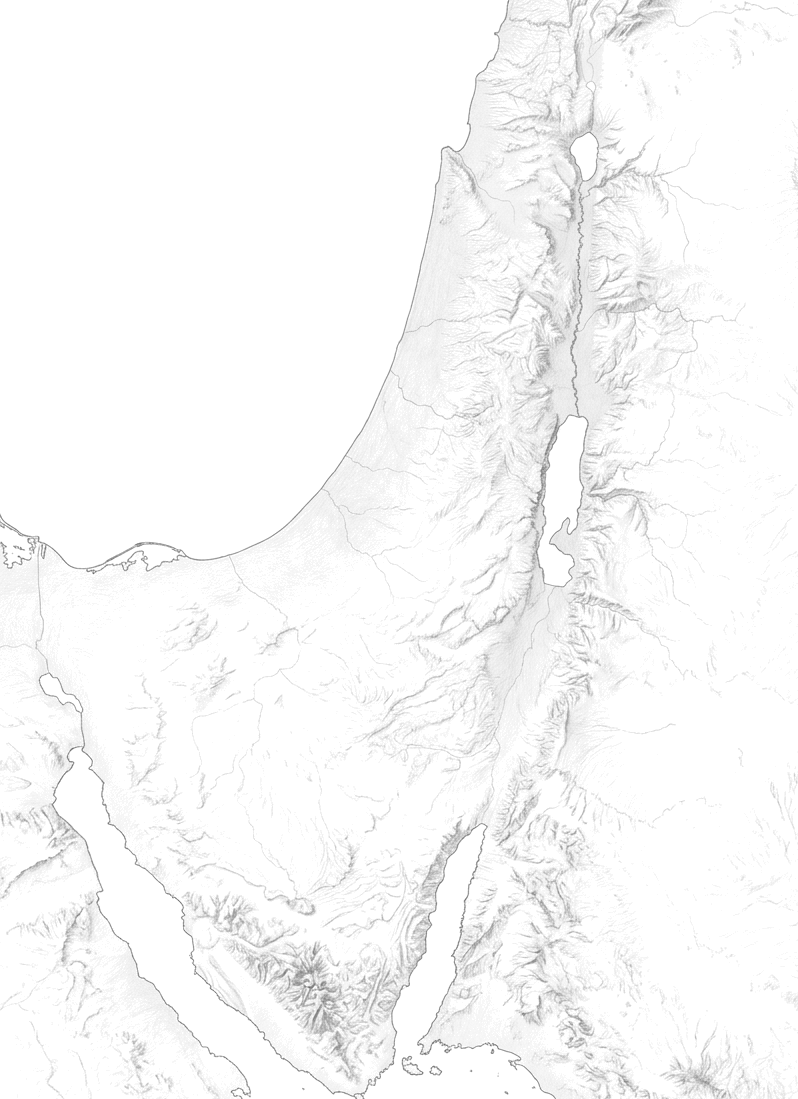
\includegraphics[width=0.87\linewidth]{theology/mariology/ark-of-the-covenant/artwork/ark-journey-map-graphite.png}};
  \begin{scope}[x={(map.south east)}, y={(map.north west)}]
    % Subtle geographic water & terrain labels
    \node[font=\scriptsize\itshape, text=black!55, align=center] at (0.390, 0.605) {Mediterranean\\Sea};
    \node[font=\tiny\itshape, text=black!55, rotate=-56] at (0.21, 0.16) {Gulf of Suez};
    \node[font=\tiny\itshape, text=black!55, rotate=74] at (0.565, 0.15) {Gulf of Aqaba};
    \node[font=\tiny\itshape, text=black!55] at (0.31, 0.29) {Sinai Peninsula};
    \node[font=\tiny\itshape, text=black!55, rotate=87] at (0.706, 0.540) {Dead Sea};
    \node[font=\tiny\itshape, text=black!55, anchor=west] at (0.755, 0.86) {Sea of Galilee};

    % Regional dashed zoom box covering Philistia, Shiloh, and Central Judah
    \draw[draw=black!75, densely dashed, line width=0.5pt] (0.49, 0.56) rectangle (0.77, 0.75);

    % Wilderness corridor (dashed: unlocated exact route)
    \draw[draw=black!85, dashed, line width=0.95pt, -{Stealth[length=2.1mm]}]
      (0.40, 0.11) .. controls (0.42, 0.25) and (0.45, 0.34) .. (0.47, 0.41);
    \draw[draw=black!85, dashed, line width=0.95pt, -{Stealth[length=2.1mm]}]
      (0.47, 0.41) .. controls (0.62, 0.40) and (0.74, 0.48) .. (0.755, 0.615);
    \draw[draw=black, line width=0.95pt, -{Stealth[length=1.9mm]}]
      (0.755, 0.615) -- (0.722, 0.646);

    % Mary's Visitation route: double white-cored line from Nazareth to Hill Country of Judea with arrowhead & hollow terminus
    \draw[draw=black, line width=1.65pt, -{Stealth[length=2.0mm]}]
      (0.660, 0.845) .. controls (0.640, 0.79) and (0.635, 0.72) .. (0.648, 0.618);
    \draw[draw=white, line width=0.7pt]
      (0.660, 0.845) .. controls (0.640, 0.79) and (0.635, 0.72) .. (0.647, 0.628);
    \filldraw[fill=white, draw=black, line width=0.65pt] (0.648, 0.612) circle (1.9pt);

    % Regional station markers
    \filldraw[fill=white, draw=black, line width=0.7pt] (0.40, 0.11) circle (2.2pt);
    \node[font=\scriptsize\bfseries, fill=white, inner sep=1pt, anchor=east] at (0.38, 0.11) {Sinai / Horeb};
    \node[font=\tiny\itshape, fill=white, inner sep=0.8pt, anchor=east] at (0.38, 0.085) {(trad. massif)};

    \filldraw[fill=white, draw=black, line width=0.7pt] (0.47, 0.41) circle (2.0pt);
    \node[font=\scriptsize, fill=white, inner sep=1pt, anchor=east] at (0.45, 0.415) {Kadesh-barnea};
    \node[font=\tiny\itshape, fill=white, inner sep=0.8pt, anchor=east] at (0.45, 0.39) {(wilderness station)};

    \filldraw[fill=black, draw=black] (0.660, 0.845) circle (2.2pt);
    \node[font=\scriptsize\bfseries, fill=white, inner sep=1pt, anchor=east, align=right] at (0.645, 0.855)
      {Nazareth\\[-0.2em]{\normalfont\tiny\itshape (Annunciation, Lk 1:26)}};

    \node[font=\tiny\itshape, fill=white, inner sep=1pt, align=center] at (0.61, 0.485) {Wilderness\\wandering\\(Num 10--33)};

    % Zoomed Detail Inset in the open upper-left Mediterranean quadrant
    \node[anchor=north west, inner sep=0, draw=black, line width=0.55pt, fill=white] (inset) at (0.012, 0.965)
      {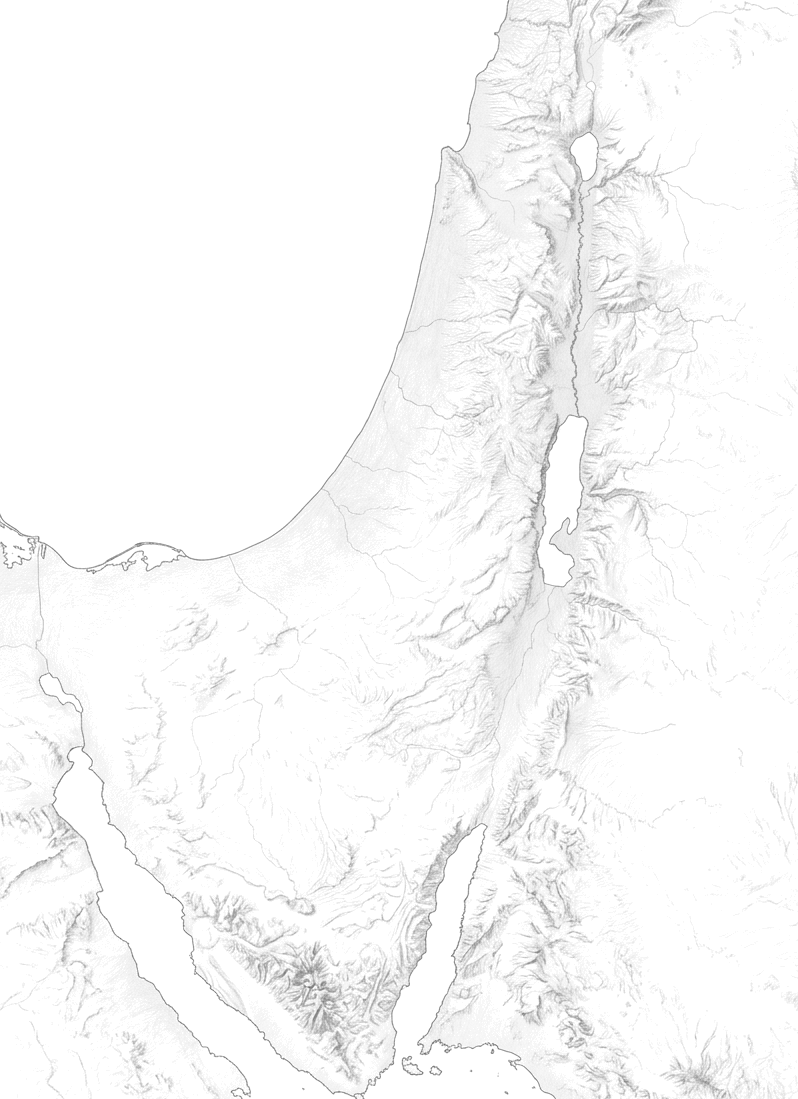
\includegraphics[trim=391bp 615bp 184bp 275bp, clip, width=0.385\linewidth]{theology/mariology/ark-of-the-covenant/artwork/ark-journey-map-graphite.png}};

    % Inset title cleanly above the top border of the inset
    \node[font=\scriptsize\bfseries, fill=white, inner sep=1.5pt, anchor=south west]
      at (0.012, 0.968) {Detail: Philistia, Shiloh, and Judah};

    % Leader connectors from inset corners to regional zoom box
    \draw[draw=black!50, densely dotted, line width=0.45pt] (inset.north east) -- (0.49, 0.75);
    \draw[draw=black!50, densely dotted, line width=0.45pt] (inset.south east) -- (0.49, 0.56);

    % Compact Legend tucked wholly inside open white Mediterranean space (explicit 1cm inner units!)
    \node[anchor=north west, draw=black!65, fill=white, line width=0.4pt, inner sep=4pt, align=left, font=\tiny]
      at (0.012, 0.625) {%
        \textbf{Map Key}\\[0.2em]
        \tikz[x=1cm,y=1cm,baseline=-0.5ex]\draw[line width=0.85pt,-{Stealth[length=1.6mm]}](0,0)--(0.55,0); Narrated Ark movement\\
        \tikz[x=1cm,y=1cm,baseline=-0.5ex]\draw[dashed,line width=0.85pt,-{Stealth[length=1.6mm]}](0,0)--(0.55,0); Unlocated / wilderness leg\\
        \tikz[x=1cm,y=1cm,baseline=-0.5ex]{\draw[line width=1.4pt](0,0)--(0.55,0);\draw[white,line width=0.6pt](0,0)--(0.55,0);} Visitation ascent (Lk 1:39)\\
        \tikz[x=1cm,y=1cm,baseline=-0.5ex]\filldraw[black](0,0) circle (1.5pt); Attested / anchored site\\
        \tikz[x=1cm,y=1cm,baseline=-0.5ex]\filldraw[fill=white,draw=black,line width=0.6pt](0,0) circle (1.5pt); Traditional / unlocated site\\
        \textit{Note:} Brenton LXX reads Ashkelon\\
        at 1 Sam 5:10 (MT/Vg: Ekron).
      };
  \end{scope}

  % Overlay routes and labels inside the zoomed Central Judah & Philistia inset
  \begin{scope}[shift={(inset.south west)}, x={(inset.south east)}, y={(inset.north west)}]
    % Narrated Conquest & Shiloh legs (Jordan -> Jericho -> Ebal -> Shiloh -> Aphek)
    \draw[draw=black, line width=0.8pt, -{Stealth[length=1.6mm]}] (0.829, 0.453) -- (0.750, 0.432);
    \draw[draw=black, dashed, line width=0.7pt, -{Stealth[length=1.5mm]}] (0.750, 0.432) -- (0.614, 0.874);
    \draw[draw=black, dashed, line width=0.7pt, -{Stealth[length=1.5mm]}] (0.614, 0.874) -- (0.636, 0.674);
    \draw[draw=black, line width=0.8pt, -{Stealth[length=1.6mm]}] (0.636, 0.674) -- (0.339, 0.642);

    % Philistine circuit (Aphek -> Ashdod -> Gath -> Ekron -> Beth-shemesh -> Kiriath-jearim)
    \draw[draw=black, line width=0.8pt, -{Stealth[length=1.6mm]}] (0.339, 0.642) -- (0.161, 0.305);
    \draw[draw=black, line width=0.8pt, -{Stealth[length=1.6mm]}] (0.161, 0.305) -- (0.268, 0.200);
    \draw[draw=black, line width=0.8pt, -{Stealth[length=1.6mm]}] (0.268, 0.200) -- (0.314, 0.395);
    \draw[draw=black, line width=0.8pt, -{Stealth[length=1.6mm]}] (0.314, 0.395) -- (0.411, 0.305);
    \draw[draw=black, line width=0.8pt, -{Stealth[length=1.6mm]}] (0.411, 0.305) -- (0.529, 0.358);

    % Davidic ascent (Kiriath-jearim -> Obed-edom -> Zion/Jerusalem)
    \draw[draw=black, line width=0.9pt, -{Stealth[length=1.6mm]}] (0.529, 0.358) -- (0.571, 0.326);
    \draw[draw=black, line width=0.9pt, -{Stealth[length=1.6mm]}] (0.571, 0.326) -- (0.636, 0.337);

    % Visitation southern approach entering inset from north to Hill Country (trad. Ein Karem)
    \draw[draw=black, line width=1.35pt, -{Stealth[length=1.6mm]}]
      (0.555, 0.995) .. controls (0.562, 0.74) and (0.572, 0.50) .. (0.579, 0.275);
    \draw[draw=white, line width=0.55pt]
      (0.555, 0.995) .. controls (0.562, 0.74) and (0.572, 0.50) .. (0.578, 0.285);

    % Station dots (filled = anchored, hollow = unlocated/tradition)
    \foreach \px/\py in {0.829/0.453, 0.750/0.432, 0.614/0.874, 0.636/0.674, 0.339/0.642, 0.161/0.305, 0.268/0.200, 0.314/0.395, 0.411/0.305, 0.529/0.358, 0.636/0.337} {
      \filldraw[fill=black, draw=black] (\px, \py) circle (1.6pt);
    }
    \filldraw[fill=white, draw=black, line width=0.65pt] (0.571, 0.326) circle (1.7pt);
    \filldraw[fill=white, draw=black, line width=0.65pt] (0.579, 0.263) circle (1.7pt);
    \filldraw[fill=white, draw=black, line width=0.65pt] (0.946, 0.289) circle (1.7pt);

    % Clean non-overlapping labels with crisp hairline pointers
    \node[font=\tiny\bfseries, fill=white, inner sep=0.7pt, anchor=west] at (0.635, 0.895) {Ebal \& Gerizim};
    \node[font=\tiny\bfseries, fill=white, inner sep=0.7pt, anchor=west] at (0.662, 0.690) {Shiloh};
    \node[font=\tiny, fill=white, inner sep=0.7pt, anchor=south] at (0.339, 0.675) {Aphek / Ebenezer};
    \node[font=\tiny, fill=white, inner sep=0.7pt, anchor=west] at (0.032, 0.245) {Ashdod};
    \draw[draw=black!60, line width=0.35pt] (0.125, 0.260) -- (0.155, 0.299);
    \node[font=\tiny, fill=white, inner sep=0.7pt, anchor=north] at (0.255, 0.172) {Gath};
    \node[font=\tiny, fill=white, inner sep=0.7pt, anchor=south] at (0.298, 0.422) {Ekron};
    \node[font=\tiny, fill=white, inner sep=0.7pt, anchor=north] at (0.405, 0.275) {Beth-shemesh};
    \node[font=\tiny, fill=white, inner sep=0.7pt, anchor=south] at (0.465, 0.455) {Kiriath-jearim};
    \draw[draw=black!60, line width=0.35pt] (0.495, 0.443) -- (0.526, 0.365);

    \node[font=\tiny\bfseries, fill=white, inner sep=0.7pt, anchor=south west] at (0.652, 0.358) {Jerusalem / Zion};
    \node[font=\tiny\itshape, fill=white, inner sep=0.7pt, anchor=east] at (0.97, 0.165) {Obed-edom (unlocated)};
    \draw[draw=black!60, line width=0.35pt] (0.640, 0.182) -- (0.573, 0.315);
    \node[font=\tiny\itshape, fill=white, inner sep=0.7pt, anchor=north] at (0.455, 0.088) {Hill Country (trad. Ein Karem)};
    \draw[draw=black!60, line width=0.35pt] (0.515, 0.105) -- (0.574, 0.252);

    \node[font=\tiny, fill=white, inner sep=0.7pt, anchor=south] at (0.768, 0.492) {Jericho};
    \draw[draw=black!60, line width=0.35pt] (0.765, 0.480) -- (0.753, 0.439);
    \node[font=\tiny, fill=white, inner sep=0.7pt, anchor=west] at (0.838, 0.530) {Jordan};
    \draw[draw=black!60, line width=0.35pt] (0.848, 0.518) -- (0.831, 0.460);
    \node[font=\tiny\itshape, fill=white, inner sep=0.7pt, anchor=north east] at (0.985, 0.255) {Mt. Nebo};
  \end{scope}
\end{tikzpicture}
\end{center}\nopagebreak[4]
\else
\begin{studybox}{Plate V: Regional Map and Central Judah Detail}
A portrait shaded-relief map spans the Sinai Peninsula, the Gulfs of Suez and Aqaba, the Dead Sea and Jordan Rift, the Philistine coastal plain, the central hill country of Judah and Samaria, and Lower Galilee around Nazareth and the Sea of Galilee. A dashed wilderness line runs north from the traditional Sinai massif through Kadesh-barnea toward the Transjordan plateau opposite Jericho. A magnified inset over the open Mediterranean quadrant details the central stations: the Jordan crossing at Gilgal, Jericho, Mounts Ebal and Gerizim, Shiloh, Aphek/Ebenezer, the Philistine circuit through Ashdod, Gath, and Ekron (noting Brenton's Septuagint reading Ashkelon at 1 Sam 5:10), the ascent through Beth-shemesh and Kiriath-jearim, the unlocated Judean house of Obed-edom, and Mount Zion in Jerusalem. A distinct white-cored double line traces Mary's Visitation ascent from Nazareth southward to the unnamed hill-country town of Judah (traditionally identified with Ein Karem), while Mount Nebo stands east of the northern Dead Sea as the horizon of 2 Maccabees 2:4.
\end{studybox}
\fi

\begin{platecaption}
\textbf{Plate V. Topographic Study of the Ark's Journey and the Visitation.} The monochrome relief base illustrates regional topography from Sinai to Galilee; route lines connect narrative stations in Scripture and do not represent recovered ancient highways. Solid circles denote established geographic anchors; hollow circles denote sites whose exact locations remain traditional or unlocated in Scripture (Sinai massif, Kadesh-barnea, Obed-edom's house, the unnamed Judean town of Luke 1:39, and the concealed cave associated with Mount Nebo in 2 Macc 2:4). Following the Hebrew and Vulgate text at 1 Sam 5:10, the Philistine leg passes through Ekron; Brenton's Septuagint reads Ashkelon.
\end{platecaption}

\subsection{Complete Station-by-Station Textual Itinerary}

The table below orders every station narrated for the earthly Ark and sets it beside the New-Covenant stations of the Incarnation and Visitation.

\begin{fourstable}{Station}{Scripture}{Geographic Status}{Role in the Covenant Arc}
1.~Mount Sinai (Horeb) &
Exod 25:10--22; 37:1--9; 40:32--36 [34--38] &
Traditional identification in southern Sinai massif; exact peak debated. &
Construction of the Ark and Tabernacle; the glory-cloud overshadows the Tent of Meeting. \\
\addlinespace[0.3em]
2.~Wilderness March and Kadesh &
Num 4:5--15; 10:33--36; 14:44 &
Wilderness transit corridor across Sinai and Negev; exact camp paths unrecovered. &
Kohathites bear the shrouded Ark three days ahead to seek a resting place; Moses cries ``Arise, O Lord.'' \\
\addlinespace[0.3em]
3.~Jordan Crossing and Gilgal &
Josh 3:3--17; 4:7--11, 19 &
Lower Jordan plain northeast of Jericho; exact ford unlocated. &
Floodwaters heap up at the touch of the priests' feet; the Ark stands in the dry bed until Israel crosses. \\
\addlinespace[0.3em]
4.~Jericho &
Josh 6:4--16 &
Anchored at Tell es-Sultan in the Jordan valley. &
Sevenfold procession of the Ark and trumpets brings down the fortified walls. \\
\addlinespace[0.3em]
5.~Mounts Ebal and Gerizim &
Josh 8:30--35 &
Anchored flanking Shechem in the central hill country. &
Israel stands on either side of the Ark as Joshua reads the blessings and curses of the law. \\
\addlinespace[0.3em]
6.~Shiloh (and Bethel variant) &
Josh 18:1; Judg 20:18, 26--28; 1 Sam 1--4 &
Anchored at Khirbet Seilun in Ephraim. MT/LXX Judg 20 places the assembly at Bethel; CV/DR identify 20:18 as Shiloh. &
First settled highland sanctuary; Samuel ministers beside the Ark until its presumptuous removal into battle. \\
\addlinespace[0.3em]
7.~Aphek and Ebenezer &
1 Sam 4:1--11 &
Western piedmont / Sharon border; battleground anchor near Tel Aphek. &
Defeat of Israel, capture of the Ark, death of Eli and his sons, and the cry \textit{Ichabod}. \\
\addlinespace[0.3em]
8.~Ashdod, Gath, and Ekron &
1 Sam 5:1--12; 6:16--17 &
Philistine pentapolis anchors (Ashdod, Tell es-Safi/Gath, Tel Miqne/Ekron). Brenton LXX reads Ashkelon at 5:10 and 6:16. &
Dagon falls shattered before the Ark; plagues compel the Philistine lords to return it with guilt offerings. \\
\addlinespace[0.3em]
9.~Beth-shemesh &
1 Sam 6:9--21 &
Anchored at Tel Beth-Shemesh in the Sorek valley ascending toward Judah. &
Milk cows draw the cart straight to Levitical territory; irreverent gazing brings sudden judgment. \\
\addlinespace[0.3em]
10.~Kiriath-jearim (Baale-Judah) &
1 Sam 7:1--2; 2 Sam 6:2--4; 1 Chr 13:5--6 &
Anchored on the western Judean ridge (Deir el-Azar / Abu Ghosh). &
Twenty years of quiet custody in the house of Abinadab on the hill under his son Eleazar. \\
\addlinespace[0.3em]
11.~Perez-Uzzah and House of Obed-edom &
2 Sam 6:6--12; 1 Chr 13:9--14 &
Exact houses and threshing floor unlocated along the ridge approach to Jerusalem. &
Uzzah dies touching the cart-borne Ark; Obed-edom's household is richly blessed for three months. \\
\addlinespace[0.3em]
12.~David's Tent on Mount Zion &
2 Sam 6:12--19; 1 Chr 15--16 &
City of David ridge south of the later Temple platform in Jerusalem. &
Levites bear the Ark on their shoulders amid shouts, sacrifice, and David's dance into the royal tent. \\
\addlinespace[0.3em]
13.~Solomon's Temple (\textit{debir}) &
1 Kgs 6--8; 2 Chr 5; 35:3 &
Temple Mount in Jerusalem. &
Ark enters beneath the monumental cherubim with only the two tablets inside; last commanded under Josiah. \\
\addlinespace[0.3em]
14.~Mount of Moses (Nebo) &
2 Macc 2:1--8; Deut 34:1 &
Transjordan ridge overlooking the Dead Sea; cave explicitly declared unknown. &
Tradition of Jeremiah concealing the Ark until God gathers His people in mercy; earthly itinerary ends here. \\
\addlinespace[0.3em]
15.~Nazareth to Hill Country of Judea &
Luke 1:26--56 &
Nazareth anchored in Lower Galilee; Luke leaves the Judean town unnamed (Christian tradition identifies Ein Karem, west of Jerusalem). &
The Spirit overshadows the Virgin; bearing the incarnate Lord, she ascends in haste, awakens John's leap and Elizabeth's cry, and remains about three months. \\
\addlinespace[0.3em]
16.~Opened Temple in Heaven &
Rev 11:19--12:6 &
Eschatological and heavenly horizon, not a terrestrial coordinate. &
The Ark of the Covenant appears in the opened heavenly temple, immediately followed by the Woman clothed with the sun. \\
\end{fourstable}
